\documentclass[a4paper, 12pt]{article}

\usepackage[utf8]{inputenc}
\usepackage[T2A]{fontenc}
\usepackage[english,russian]{babel}

\usepackage{amsmath,amssymb,amsthm}

\usepackage{biblatex}
\usepackage{hyperref}

\usepackage{graphicx}
\usepackage{tikz-cd}
\usepackage[a4paper,hmargin=2.5cm,vmargin=2.5cm]{geometry}

\usepackage{enumitem}


\addbibresource{refs.bib}


\newtheorem*{theorem}{Теорема}
\newtheorem{mtheorem}{Теорема}
\newtheorem*{lemma}{Лемма}

\theoremstyle{definition}
\newtheorem{definition}{Определение}
\newtheorem{remark}{Замечание}

\def\keywords#1{\begin{center}{\bf Ключевые слова}\\\textit{#1}\end{center}} %


\author{\large Дьяконов Фёдор Юрьевич \\ [1cm]{\small Научный руководитель: Рябичев Андрей Дмитриевич}}


\title{
Гомологии трёхмерных многообразий
}

% \date{11 июня 2023 г.}
\date{}

\begin{document}

\maketitle

\keywords{3-многообразия, гомологические сферы, копредставления групп}

\begin{abstract}
    В этой работе освещается построение гомологической 3-сферы. Для этого мы предварительно упрощаем задачу до построения 3-многообразия с совершенной фундаментальной группой. Далее при помощи вычислительных методов мы находим сбалансированное задание некоторой такой группы образующими и соотношениями, что позволяет сконструировать по нему многообразие при помощи разбиения Хегора.
\end{abstract}


\section{Введение}
    Анри Пуанкаре, заложивший основы алгебраической топологии, занимался поиском исчерпывающего набора инвариантов, которые бы различали сферы. После того, как он ввёл один из них, эквивалентый гомологиям в современном определении, он с удивлением обнаружил, что в размерности 3 этот инвариант не является достаточным.

    \begin{theorem}[Пуанкаре]
        Существует трёхмерное многообразие, гомологические и когомологические группы которого такие же, как и у $\mathbb{S}^3$.
    \end{theorem}

    Многообразие с таким свойством мы будем называть \textit{гомологической 3-сферой}. Целью нашей работы является явное построение такого многообразия, исходящее лишь из определяющего его свойства. Хотя существование гомологических сфер давно и широко известно \cite[Глава 6, \S18]{1997-hj}, способ, представленный нами, был выработан оригинально. Его определяющая черта заключается в том, что он позволяет совершить большую часть работы на компьютере.

    Для того, чтобы упростить задачу построения такого многообразия, мы предварительно введем несколько теорем. Более точно, задача сведется к поиску 3-многообразия, фундаментальная группа которого совершенна. Напомним при этом, что группа называется \textit{совершенной}, когда её абелианизация тривиальна. В размерности 3 это условие оказывается достаточным, чтобы определить все гомологические и когомологические группы пространства, что описывается в \S2. Далее в \S3 мы показываем, как при помощи подходящего задания совершенной группы образующими и соотношениями можно сконструировать такое многообразие. И, наконец, в \S4 мы находим такую группу при помощи вычислительных методов и в \S4-5 явно представляем конструкцию искомой гомологической сферы.



\section{Предварительные алгебраические утверждения}

    \subsection{Базовые факты алгебраической топологии}
        Чтобы связать младшие гомотопическую и гомологическую группы, мы возпользуемся следующим известным \cite[Chapter~2,~Section~2.A]{Hatcher2001-hm} утверждением:

        \begin{theorem}[Гуревич]
            Для линейно связного топологического пространства $X$ верно, что
                 \begin{equation*} H_1(X, \mathbb{Z}) \cong \pi_1(X)_{ab}, \end{equation*}
            где последнее обозначает абелианизацию фундаментальной группы $X$.
        \end{theorem}
    
        Далее, для вычисления остальных гомологических и когомологических групп через известные нам, мы введем еще две теоремы (\cite[Chapter~3,~Section~3.3]{Hatcher2001-hm}, \cite[Chapter~3,~Section~3.1]{Hatcher2001-hm}):

        \begin{theorem}[Двойственность Пуанкаре]
            Для связного ориентируемого $n$-многообразия $M$ существует изоморфизм между его группами когомологий и гомологий:
                \[ \begin{tikzcd}
                     H^k(M, \mathbb{Z}) \arrow{r}[label]{\sim} & H_{n - k}(M, \mathbb{Z}) 
                \end{tikzcd} \]
        \end{theorem}

        \begin{theorem}[Oб универсальных коэффициентах для когомологий]
            Пусть дан цепной комплекс свободных абелевых групп $C_\bullet$, и его группы гомологий (над $\mathbb{Z}$) обозначены через $H_n$. Тогда существует и расщепляется точная последовательность
                \[ \begin{tikzcd}
                    0 \arrow{r} & \textnormal{Ext}(H_{n - 1}(C_\bullet), \mathbb{Z}) \arrow{r} & H^n(C_\bullet) \arrow{r} & \textnormal{Hom}(H_n(C_\bullet), \mathbb{Z}) \arrow{r} & 0 
                \end{tikzcd} \]
        \end{theorem}

    % \pagebreak
    \subsection{Следствия}

        \begin{lemma}
            Линейно связное ориентируемое замкнутое 3-многообразие $M$ является гомологической сферой, если его фундаментальная группа совершенна. 
        \end{lemma}

        \begin{proof}
            В силу теоремы Гуревича совершенность $\pi_1(M)$ (то есть тривиальность $\pi_1(M)_{ab}$) равносильна тому, что $H_1(M) = 0$. Отсюда следует, что в обратную сторону утверждение верно. Докажем его в другую сторону.
                        
            $M$ линейно связно, ориентируемо и замкнуто. Значит, $H_0(M) = H^0(M) = \mathbb{Z}$, и также $H^3(M) = H_3(M) = \mathbb{Z}$. 
                      
            Докажем далее, что его первые когомологии тоже ноль, запишем формулу универсальных коэффициентов:


                \[ \begin{tikzcd}
                    0 & {\textnormal{Ext}(H_0(M), \mathbb{Z}) } \arrow[draw=none]{d}[marking]{\cong} & {H^1(M)} & {\textnormal{Hom}(H_1(M), \mathbb{Z})) } \arrow[draw=none]{d}[marking]{\cong} & 0 \\
                    & {\textnormal{Ext}(\mathbb{Z}, \mathbb{Z}) = 0} & & \textnormal{Hom}(0, \mathbb{Z}) = 0,
                    \arrow[from=1-1, to=1-2]
                    \arrow[from=1-2, to=1-3]
                    \arrow[from=1-3, to=1-4]
                    \arrow[from=1-4, to=1-5]
                    % \arrow[from=1-2, to=2-3]
                \end{tikzcd} \]
            то есть мы получим, что $H^1(M) = 0 \oplus 0 = 0$. 
    
            Отсюда при применении двойственности Пуанкаре к нулевым $H_1(M)$ и $H^1(M)$ сразу следует, что также \[H_2(M) = H_1(M) = 0,\]
            что завершает перечисление всех интересующих нас (ко)-гомологических групп.
        \end{proof}

\section{Некоторые конструкции из маломерной топологии}

    \subsection{Определения}
    
        В интересах построения трехмерных многообразий мы воспользуемся инструментами, подробно описанными в \cite[Глава 4]{1997-hj}, здесь же мы кратко опишем основные определения. 

        \begin{definition}
            \textit{Разбиением Хегора} ориентируемого трехмерного многообразия $M$ называют его представление в виде объединения двух тел с ручками $M_1^3$ и $M_2^3$ с общей границей $\partial M_1^3 = \partial M_2^3$, отождествленной по некоторому гомеоморфизму.
        \end{definition}

        \begin{definition}
            \textit{Диаграммой Хегора} называют систему замкнутых ориентированных простых кривых $u_1, \dots, u_g$ и $v_1, \dots, v_g$ на сфере с $g$ ручками, которые удовлетворяют следующим условиям: 
            \begin{enumerate}[label=(\roman*)]
                \item кривые $u_i$ попарно не пересекаются и дополнение к их объединению связно;
                \item кривые $v_i$ попарно не пересекаются и дополнение к их объединению связно.
            \end{enumerate}
        \end{definition}

        При этом по разбиению Хегора можно сконструировать многие диаграммы Хегора. А именно: рассмотрим, например, стандартные (при вложении в $\mathbb{R}^3$) системы меридианов $u_1, \dots, u_g$ на $\partial M^3_1$ и $v_1, \dots, v_g$ на $\partial M^3_2$. Тогда на $\partial M^3_2$ система кривых из $v_1, \dots, v_g$ и $f(u_1), \dots, f(u_g)$ будет являться такой диаграммой.

        Диаграммы Хегора удобны для явного задания, и благодаря следующему утверждению \cite[Глава 4, \S 10.3]{1997-hj} также позволяют конструировать трёхмерные многооборазия, чем мы и будем пользоваться дальше: 

        \begin{theorem}
            Для каждой диаграммы Хегора существует гомеоморфизм сферы с $g$ ручками в себя, который переводит первый набор кривых ($u_1, \dots, u_g$) во второй ($v_1, \dots, v_g$). Это позволяет сконструировать разбиение Хегора, приклеив границы двух тел с $g$ ручками по этому гомеоморфизму. При этом для любых подходящих гомеоморфизмов результирующие из разбиения многообразия будут гомеоморфны.
        \end{theorem}

    \subsection{Фундаментальная группа 3-многообразия \\ с данным разбиением Хегора}

        Чтобы контролировать алгебраические инварианты искомого многообразия, мы воспользуемся следующей теоремой:

        \begin{theorem} 
            Пусть для $M$ задано разбиение Хегора на два тела с ручками рода $g$. Тогда у фундаментальной группы $M$ существует сбалансированное копредставление с $g$ образующими и $g$ соотношениями.
        \end{theorem}

        Напомним, что \textit{сбалансированным копредставлением} группы называется ее задание образующими и соотношениями, при котором их число совпадает.

        \begin{proof}
            Предположим, что $M$ разбито на тела $M_1$ и $M_2$ по гомеоморфизму $f: \partial M_1 \rightarrow \partial M_2$. Мы покажем, что $\pi_1(M)$ совпадает с фундаментальной группой линейно связного CW-комплекса, который содержит $g$ одномерных клеток и $g$ двумерных клеток.  
            
            Рассмотрим $g$ меридианов $w_1, \dots, w_g$ на $M_1$, которые ограничивают диски $D_1, \dots, D_g$ внутри тела.

            Заметим, что $M \cong M_1 \cup_f M_2$, а дополнение к $\bigsqcup_{i = 1}^{g} D_i$ во внутренности $M_1$ гомеоморфно трёхмерному диску. Поскольку $M$ можно считать клеточным комплексом, то этой трёхмерной клеткой можно принебречь при вычислении фундаментальной группы: 
            \[\pi_1(M) \cong \pi_1 \left( \left(\bigsqcup_{i = 1}^{g} D_i\right) \cup_f M_2 \right),\] 
            где в правой части написано многообразие без этого внутреннего трёхмерного диска.
            
            В свою очередь, $M_2$ деформационно ретрагируется на букет $g$ окружностей, назовём эту ретракцию $\rho$. Тогда


            \[\pi_1(M) \cong \pi_1\left( \left(\bigsqcup_{i = 1}^{g} D_i\right) \cup_{\rho \circ f} \bigvee_{j = 1}^{g} \mathbb{S}^1\right) \]

            Где справа и написано клеточное пространство с одной нульмерной клеткой, $g$ одномерными клетками и $g$ двумерными клетками. Эти двумерные клетки будут приклеены по характеристическим отображениям, которые получаются ограничением $\rho \circ f$ на $w_i$. Тогда по теореме о фундаментальной группе клеточного комплекса это и даст нам искомое копредставление. 
            
        \end{proof}

        \begin{remark}{}
            \label{fgroup}
            Более того, если это разбиение Хегора было получено из диаграммы Хегора, в которой первый набор кривых был выбран как меридианы на $M_1$, то соотношения в полученной группе будут определены образами второго набора кривых при ретракции, чем мы и воспользуемся далее.
        \end{remark}
        
\section{Обзор использованных вычислительных методов}     
    Чтобы найти совершенную группу и некоторое ее сбалансированное копредставление, мы выбрали подход перебора таких копредставлений и затем проверки свойств полученных групп.

    В общем проблема доказательства тривиальности группы по ее копредставлению алгоритмически неразрешима \cite{Rabin1958}. Проверка тривиальности её абелианизации при этом весьма проста в силу следующего утверждения:

    \begin{lemma}
        Пусть группа $G$ задана копредставлением $\langle e_1, e_2, \dots e_n \mid w_1, w_2, \dots, w_n \rangle$ c $n$ образующими и $n$ соотношениями, длина которых (то есть сокращенная запись из символов $e_i$ и $e_i^{-1}$) не превосходит $l$.
        
        Тогда тривиальность ее абелианизации $G_{ab}$ можно установить за временную сложность $O(n l + f(n))$, где $f(n)$ обозначает асимптотику работы алгоритма поиска определителя квадратной матрицы размера $n$, то есть, например, $O(n^3)$.
    \end{lemma}

    \begin{proof}
        По аналогии с соотношениями в задании $G$ запишем соотношения в её абелианизации. Для этого переставим и сократим образующие и получим слова, которые будут иметь вид $e_1^{\alpha_{i, 1}} e_2^{\alpha_{i, 2}} \dots e_n^{\alpha_{i, n}}$. Итоговая группа тогда изоморфна фактору $\mathbb{Z}^n$ по целочисленной решетке, порожденной векторами, полученными из этих слов.

        Запишем эти вектора как столбцы в целочисленную матрицу $A$. Воспользуемся теоремой о существовании нормальной формы Смита у матрицы над кольцом главных идеалов \cite[Chapter 3, Theorem 7.9]{Lang2002}. По ней для этой матрицы $A$ существуют такие обратимые целочисленные матрицы $P$ и $Q$, что $D = P A Q$ -- диагональная матрица. При этом каждый следующий диагональный элемент $D$ делится на предыдущие. В силу обратимости $P$ и $Q$ факторы $\mathbb{Z}^n$ по столбцам матрицы $A$ и по столбцам $D$ изоморфны.

        А такой фактор для $D$ тривиален тогда и только тогда, когда все диагональные элементы $D$ равны $\pm 1$. А так как все её элементы целые, то это равносильно тому, что $\det D = \pm 1$, и, значит, $\det A = \pm 1$.

        Тогда искомый алгоритм можно реализовать, сначала вычислив элементы матрицы $A$, что занимает $O(n l)$ времени, и затем посчитав определитель $A$ за сложность $O(f(n))$.
    \end{proof}

    Чтобы упростить реализацию соотношений в полученном копредставлении как системы простых кривых на сфере с $g$ ручками, мы зафиксировали $g = 2$, то есть перебор велся по двухгенераторным сбалансированным копредставлениям. При эффективном переборе это значило, что матрица предпосчитывалась в процессе генерации и имела размер 2 на 2, то есть её определитель вычислялся за постоянное время. 

    Таким образом, в процессе перебора мы за константное время узнаем, тривиальна ли абелианизация группы. Однако для каждого из них оставалась возможность того, что и сама группа тривиальна, и, значит, не подходит нам.

    Чтобы исключить такие копредставления, мы затем пользовались алгоритмом Тодда — Коксетера перечисления смежных классов группы, заданной копредставлением, по некоторой ее подгруппе (см., например, \cite[Chapter 5]{Holt2005}), который, если группа имеет достаточно малый порядок и нетривиальна, дает нам этот результат за фиксированное число операций.

    Если же за определенное число операций (то есть для достаточно малой таблицы смежных классов) мы не получали положительного результата, или получали, что группа тривиальна, мы останавливали алгоритм и переходили к следующему копредставлению. Это значит, что, вероятно, мы пропустили некоторые интересующие нас группы, однако нас интересовало построение примера, а не исчерпывающая их классификация.

    Эти вычисления производились при помощи программы на языке программирования Julia \cite{Julia-2017} с интерфейсом к системе компьютерной алгебры GAP \cite{GAP4}, в которой реализован алгоритм Тодда — Коксетера. Исходный код и результаты вычислений предоставлены в репозитории \cite{Dyakonov2023}.
    

\section{Результаты}

    \begin{figure}[h] 
        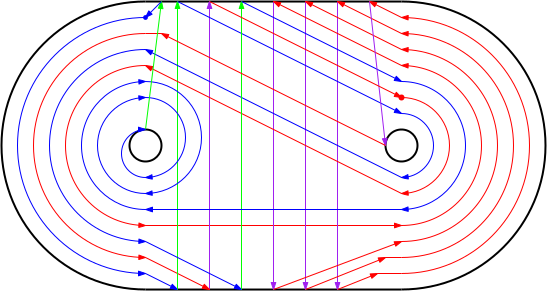
\includegraphics[width=\textwidth]{diagram} 
        \caption{Реализация соотношений как системы попарно непересекающихся простых кривых. Здесь первое соотношение соответствует кривой, обозначенной красным цветом, где пунктирная часть находится на обратной стороне поверхности. Аналогично синим цветом обозначена вторая кривая. При этом кривые попарно не пересекаются, а дополнение к ним линейно связно.}
        \label{fig_1}
    \end{figure}

    Мы перебрали все сбалансированные двухгенераторные копредставления групп, в которых длина соотношений (выраженная в терминах образующих и их обратных) хотя бы 3 и не превосходит 7.

    За приблизительно 10 минут на одном персональном компьютере это дало порядка 600 различных (с точностью до естественных симметрий) копредставлений, которые задают нетривиальную конечную совершенную группу. Все они при ближайшем рассмотрении оказались изоморфны $\textnormal{SL}_2(\mathbb{F}_5)$.

    Мы выбрали одно из них, а именно $G = \langle a, b \mid a b a^{-4} b, (b a)^2 b^{-3} \rangle$, и реализовали соотношения в нем как пунктированные кривые на сфере с двумя ручками. Эти кривые при ретракции на букет двух окруностей (стягивающей отмеченные точки на кривых в отмеченную точку букета) дадут обозначенные элементы в фундаментальной группе. 
    
    При этом порождающая $a$ в букете соответствует кривой, обходящей один раз вокруг правой (см. рисунок \ref{fig_1}) окружности (по часовой стрелке). Порождающая $b$ соответствует кривой, обходящей один раз вокруг левой окружности (против часовой стрелки).

    Полученная мультикривая удовлетворяет требованиям для одного из набора кривых диаграммы Хегора. Дополним его вторым набором, состоящим из меридианов на сфере с двумя ручками. Тогда в силу замечания \ref{fgroup} фундаментальная группа полученного 3-многообразия будет иметь копредставление $G$, то есть будет изоморфна $\textnormal{SL}_2(\mathbb{F}_5)$ и совершенна.

    Что и дает нам искомое построение.

\printbibliography

%% ===========================================================================
%%



\end{document}